%%
%% This is file `example/ch_intro.tex',
%% generated with the docstrip utility.
%%
%% The original source files were:
%%
%% install/buptgraduatethesis.dtx  (with options: `ch-intro')
%% 
%% This file is a part of the example of BUPTGraduateThesis.
%% 

\chapter{相关概念与相关技术}
本章主要针对本课题研究中涉及到的一些主要概念和相关技术进行介绍。包括本课题研究的主要问题定义以及评价指标的介绍,以及自然语言处理领域的三类基础文本表示方法的介绍,还有本课题研究内容中的两个重要的基础知识,注意力机制和多任务学习。
\section{面向司法领域多标签文本分类核心问题}
在司法领域,针对法官拟定的裁判文书,推荐可能需要引用的法条,可以为法官的工作提供便利;针对普通用户输入的案情描述,推荐可能涉及的法条,可以为普通民众提供一定的法律支持。本课题主要研究面向司法领域的多标签分类问题,本节从问题定义和评价指标两个方面进行介绍。
\subsection{面向司法领域多标签分类的问题定义}


给定事实描述,对于法官来说,一种通用的处理方法是他们首先浏览所有的法条,之后根据对案情描述的分析,得到被告人触犯了哪些法条。由于法条数量多而繁杂,因此快速定位相关法条是非常困难的。如表\ref{t:example}所示,事实描述是一段描述被告人的案情介绍或者事实证据,该被告人触犯了刑法第二百六十四条以及刑法第二百三十二条。本课题面向司法领域的多标签分类问题是以事实描述为输入,预测被告人可能涉及了哪些法条。
\begin{table}[hbt]
    \caption{判决文书样例}
    \label{t:example}
    \centering
    \begin{tabular}{lp{12cm}p{7cm}}
    \hline
    \textbf{事实描述}: &\emph{被告人温某1供称因孙某某(被害人,女,殁年47岁)借钱不还,遂产生杀害孙某某之念。2015年6月18日20时左右,温某1携带尖刀前往孙某某位于瓦房店市。期间,温某1持刀切割孙某某颈部,致其因创伤失血性休克死亡。嗣后,温某1从孙某某处窃取价值人民币1792元的金耳环;同时,为掩饰罪行,温某1将孙某某住处的监控主机拿走,丢弃于一水井内。2015年9月7日,温某1到瓦房店市公安局投案,并如实供述自己的犯罪事实...综上,根据被告人温某1的犯罪事实、情节及对社会的危害程度以及其犯罪行为给附带民事诉讼原告人造成的物质损失,依据《中华人民共和国刑法》...}\\
    \hline
    \textbf{相关法条}: 
    &\emph{\textbf{刑法第二百六十四条}: 盗窃公私财物,数额较大的,或者多次盗窃、入户盗窃、携带凶器盗窃、扒窃的,处三年以下有期徒刑、拘役或者管制,并处或者单处罚金;数额巨大或者有其他严重情节的,处三年以上十年以下有期徒刑,并处罚金;数额特别巨大或者有其他特别严重情节的,处十年以上有期徒刑或者无期徒刑,并处罚金或者没收财产。 \newline
    \textbf{刑法第二百三十二条}: 故意杀人的,处死刑、无期徒刑或者十年以上有期徒刑;情节较轻的,处三年以上十年以下有期徒刑。}\\
    \hline
    \end{tabular}
\end{table}
\subsection{面向司法领域多标签分类的评价指标}
多标签分类问题与单标签分类问题不同,给定一个样本,其对应的标签可能存在多个,因此在进行多标签分类评估时,需要整体考虑不同标签的影响。本课题采用基于宏平均的方法和杰卡德相似系数两种评价指标进行结果评估。
\subsubsection{基于宏平均的方法}
现有的二元评价指标以宏平均和微平均为基础,可以将样本根据真实类别和预测类别划分为:
\begin{itemize}
    \item 真正例(True Positive,TP):真实类别为正例,预测类别为正例。
    \item 假正例(False Positive,FP):真实类别为负例,预测类别为正例。
    \item 假负例(False Negative,FN):真实类别为正例,预测类别为负例。
    \item 真负例(True Negative,TN):真实类别为负例,预测类别为负例。
\end{itemize}

定义准确率($P$)和召回率($R$),及$F1$如下:
\begin{equation}
    \begin{aligned}
        &P=\frac{TP}{TP+FP}\\
        &R=\frac{TP}{TP+FN}\\
        &F1=\frac{2\times P \times R}{P+R}\\
    \end{aligned}
\end{equation}

针对一般的二分类问题,可以用以上指标进行评价,而针对多标签分类问题,每个样本包含多个标签,即每个标签都是一个二分类问题,因此,我们需要综合考虑所有标签上的结果,本课题采用宏平均的方式对实验结果进行评价,计算结果如下:

\begin{equation}
    \begin{aligned}
        & Macro\textrm{-}P &=& \frac{1}{n}\sum_{i=1}^{n}P_{i} \\
        & Macro\textrm{-}R &=& \frac{1}{n}\sum_{i=1}^{n}R_{i} \\
        & Macro\textrm{-}F1 &=& \frac{1}{n}\sum_{i=1}^{n}\frac{2\times Macro\textrm{-}P \times Macro\textrm{-}R}{Macro\textrm{-}P+Macro\textrm{-}R} \\
    \end{aligned}
\end{equation}

其中,n代表多标签分类中标签的总个数,$P_i$,$R_i$分别代表第$i$个标签的准确率,召回率,由每类标签所有样本的真实类别和预测类别进行计算。
\subsubsection{杰卡德相似系数}
杰卡德相似系数是另一种常见的多标签分类评价指标,它用来评价真实标签集合和预测标签集合之间的相似度,它由两个标签集合的交并比定义,其定义如下:

\begin{equation*}
Jaccard =\frac{1}{|X|}\sum_{i=1}^{|X|} \frac{ | Y^{(i)} \cap Y_{test}^{(i)} | } {|Y^{(i)} \cup Y_{test}^{(i)}|}
\end{equation*}
其中,$|X|$代表测试集样本个数,$Y$和$Y_{test}$分别代表预测标签集合和真实标签集合,$i$代表测试集中的第$i$个样本。

\section{文本表示方法}
文本表示方法作为文本处理的一个核心内容,一直以来都是学者们的研究重点,更有效的文本表示方法对于提高算法性能起到了至关重要的作用。现有的文本表示方法主要分为以下三种类型:
\subsection{基于空间向量的表示方法}
文本表示最直观的方式是空间向量表示法。这类方法将文本表示成文本表示为词组成的
向量,向量的每一维代表一个词的词频,向量的维度对应词表的大小,针对“丈夫借名买
车,妻子离婚,丈夫偿还。”这句话,根据预定义字典: {丈夫:0,买车:1,借名:2,偿还:3,分
割:4,夫妻:5,妻子:6,抢劫:7,支:8,离婚:9},可以得到文本向量表示如下:
\begin{eqnarray*}
[2,1,1,1,0,1,0,0,0,1]
\end{eqnarray*}
这种方式仅考虑文本中的词频信息,并不考虑不同词在文本中的重要程度,因此无法有
效表征文本。为了解决这个问题,之后出现了 $TF-IDF$ 方法, $TF-IDF$ 方法由两部分组成,即
$TF$ 和 $IDF$:
\begin{equation}
\begin{aligned}
    & TF(w_{ij},d_j)=count(w_{jk},d_j)\\
    & IDF(w_jk,d_j)=log(\frac{N}{df_{w_{jk}}})\\
    & TF\textrm{-}IDF(w_{kj,d_j})=TF(w_{jk},d_j)*IDF(w_{jk},d_j)\\
\end{aligned}
\end{equation}

其中$d_j$代表语料库中的第k个文档,$w_{jk}$代表第j个文档中的第$k$个词,$df_{w_{jk}}$代表词$w_{jk}$在整个语料库中出现的文档个数。那么词$w_{jk}$的$TF\textrm{-}IDF$值即为该词的TF值与$IDF$值之积。由上述公式可以看出,$TF$值表示某个单词在当前样本中的贡献程度, $IDF$值代表某个单词在整个语料库中不同样本的贡献程度,某些词在当前样本中出现的次数很高,即$TF$值很高,同时这些词在不同文档中出现的次数也很多,即$IDF$值很低,那么这些词对不同文本的区分度就没有那么明显,所以$IDF$值能很好弥补$TF$只关注局部的缺点。

$TF\textrm{-}IDF$这类向量空间表示法将各词之间架设为线性无关的,这造成了这类算法无法进行语义相关的判断。此外,向量的维度对应词表的大小,因此,向量维度随着词表增大而增大,由于样本的中所包含的词远远少于词表,因而造成了向量的高度稀疏。

\subsection{基于主题模型的表示方法}
为了更好地解决语义表示能力,研究者提出了潜在语义分析(LSA)方法~\cite{DeerwesterDLFH90},LSA构建文档和词的共现矩阵,通过奇异值分解对原始矩阵降维,可以得到文档向量和词向量,假设A是词\textrm{-}文档矩阵,矩阵每列对应一篇文章,每行是一个单词。 $B = A^{T}A$是 文档\textrm{-}文档矩阵,如果文档 $i$ 和文档$j$有$b$个相同的单词,则$B[i,j]=b$。 $C = AA^{T}$是词\textrm{-}词矩阵,如果单词$i$和单词$j$同时出现在一篇文档中的频率是$c$,则$C[i,j]=c$。对$A$进行SVD 分解:

\begin{equation}
    A=U\sum V^{T}
\end{equation}

其中$U$是由矩阵B的特征向量构成,$V$是由矩阵$C$的特征向量构成,$\sum$是由矩阵$B$的特征值的平方根构成的对角矩阵。保留$\sum$的前$K$个特征值,对矩阵$U$、$V$保留前$K$项:
\begin{equation}
    A_{m\times n}=U_{m\times k}{\Sigma}_{k\times k}V^{T}_{k\times n}
\end{equation}
根据上式,我们得到Term\textrm{-}Term与Document\textrm{-}Document在潜在语义空间的相关性矩阵表示:
\begin{equation}
    \begin{aligned}
        & A_{k}A^{T}_{k}=(U_{k}{\Sigma}_{k}V^{T})(U_{k}{\Sigma}_{k}V^{T})^{T}=U_{k}{\Sigma}_{k}V^{T}V_{k}\Sigma_{k}^{T}U_{k}^{T}=U_{k}\Sigma_{k}\Sigma_{k}^{T}U_{k}^{T} \\
        & A^{T}_{k}A_{k}=(U_{k}{\Sigma}_{k}V^{T})^{T}(U_{k}{\Sigma}_{k}V^{T})=V_{k}{\Sigma}_{k}U^{T}U_{k}\Sigma_{k}^{T}V_{k}^{T}=V_{k}\Sigma_{k}\Sigma_{k}^{T}V_{k}^{T} \\
    \end{aligned}
\end{equation}

因此,将$U_k\Sigma_{k}$矩阵的行看作是 term 在语义空间的表示,将$V_{K}\Sigma_{k}^{T}$的行看作是 Document 在语义空间的表示。LSA算法原理简单,一次奇异值分解就能得到向量空间表示,同时解决了词义相似性的问题。$LSA$算法通过线性代数中的奇异值分解实现文档映射到低维语义空间里的向量,但是空间中的每个维度没有明确物理含义。

在此之后,还有pLSA模型~\cite{Hofmann99}假设文档具有主题分布,尝试从概率生成角度进行文本表示,这类方法不是本文研究重点,因此此处不进行详细描述。

\subsection{基于神经网络的表示方法}
随着神经网络技术的发展,Bengio等人尝试使用神经网络进行自然语言建模\cite{BengioDV00},在此基础上,Mikolov等人提出了Word2Vec方法\cite{abs-1301-3781},采用 CBOW和Skip-gram方法,进行语言模型建模,CBOW使用上下文对目标词进行预测,Skip-gram通过目标词对上下文进行预测,在此基础上得到的词语义文本表达,在自然语言的各个领域,取得了非常好的效果。fastText~\cite{GraveMJB17}根据word2vec思想,对文本进行建模实现分类。其模型如图~\ref{fig:fasttext}所示:
\begin{figure*}[htb]
    \centering
    \includegraphics[width=12cm,height=6cm, clip=true]{./sources/fasttext.eps}
    \vspace{-10pt}
    \caption{\label{fig:fasttext} fastText模型结构图}
    \vspace{-5pt}
\end{figure*}

该模型由输入层,隐藏层和输出层组成,输入层为词向量,隐藏层通过将文本中词向量进行平均得到句子向量的表达,最后通过暑促层线性分类器进行文本分类。该方法训练速度快,在很多文本分类任务中取得了出色的表现。

随着 CNN/RNN 的研究不断增多,越来越多的模型使用这些方法对文本进行建模。 Kim 等人
提出基于卷积神经网络的文本分类方法~\cite{Kim14},其模型结构如图~\ref{fig:textcnn}所示:
\begin{figure*}[htb]
    \centering
    \includegraphics[width=12.5cm,height=5.5cm,clip=true]{./sources/textcnn.eps}
    \vspace{-10pt}
    \caption{\label{fig:textcnn} TextCNN模型结构图}
    \vspace{-5pt}
\end{figure*}

该模型由卷积层,MaxPooling层,全连接层组成,该模型通过不同大小的卷积核提取不同窗口 N-gram特征,经过MaxPooling 将不同窗口特征拼接作为文本表达,由于CNN擅长提取局部特征,仅能获取局部信息,会损失一些语义信息。针对CNN的不足之处,研究者们提出了RNN,LSTM模型,LSTM模型结果如图~\ref{fig:lstm}:
\begin{figure*}[htb]
    \centering
    \includegraphics[width=12cm,height=5cm,clip=true]{./sources/lstm2.eps}
    \vspace{-10pt}
    \caption{\label{fig:lstm} LSTM模型结构图}
    \vspace{-5pt}
\end{figure*}

LSTM,全称长短期记忆网络,是为了解决CNN等模型只能获取局部信息,无法有效获取序列长期依赖问题而提出来的,它主要包括遗忘门、输入门和输出门三部分。首先,该网络决定从前一步的细胞单元选择丢弃多少的信息,其计算过程如下:
\begin{equation}
    f_t = \sigma(W_f\dot[h_{t-1,x_t}] + b_f)
\end{equation}

其中,$h_{t-1}$代表前一步输出,$x_t$代表当前输入,$\sigma$代表sigmoid函数。

之后模型通过输入门对信息进行更新,首先通过sigmoid层决定信息的更新比例;一个tanh层生成新的状态向量。之后结合两部分内容,对细胞状态进行更新,其计算过程如下:
\begin{equation}
    \begin{aligned}
        & i_t = \sigma(W_i\dot[h_{t-1},x_t]+b_i) \\
        & \tilde{C}_t=tanh(W_C\dot[h_{t-1},x_t]+b_C)
    \end{aligned}
\end{equation}

结合前面的信息,通过下面的式子产生新的细胞状态:
\begin{equation}
    C_t=f_t*C_{t-1}+i_t*\tilde{C}_t
\end{equation}

最后,通过输出门,决定新的输出隐层状态,计算过程如下:
\begin{equation}
    \begin{aligned}
        & \sigma_t=\sigma(W_o[h_{t-1},x_t]+b_o) \\
        & h_t=o_t*tanh(C_t)\\
    \end{aligned}
\end{equation}

采用基于神经网络的文本表示方法,能有效降低文本表示维度过高的问题,并且能够获取更多的文本语义信息,因此基于神经网络的文本表示是本课题采用的主要方式。

\section{注意力机制}

注意力机制是一种广泛应用在深度学习的各个领域的机制,其本质是一种特征加权的方式,注意力在自然语言处理领域的应用最早是在机器翻译领域\cite{bahdanau2014neural},传统的机器翻译模型通常由编码器-解码器结构组成,编码层即文本表示层,采用文本表示模型对文本进行编码,将输入语句转换成文本表示向量,之后通过解码器对该向量进行解码,将该向量翻译成目标语言。最基本的编码器-解码器结构由RNN构成,RNN由于本身结构的限制,无法得到文本序列的长期依赖,因此,为了解决这个问题,机器翻译模型引入了注意力机制,通过在不同解码阶段不同词重要性的不同,对文本向量进行加权,将语义信息集中在需要的部分。最基本的注意力机制模型如图~\ref{fig:attention}所示:
\begin{figure}[htb]
    \centering
    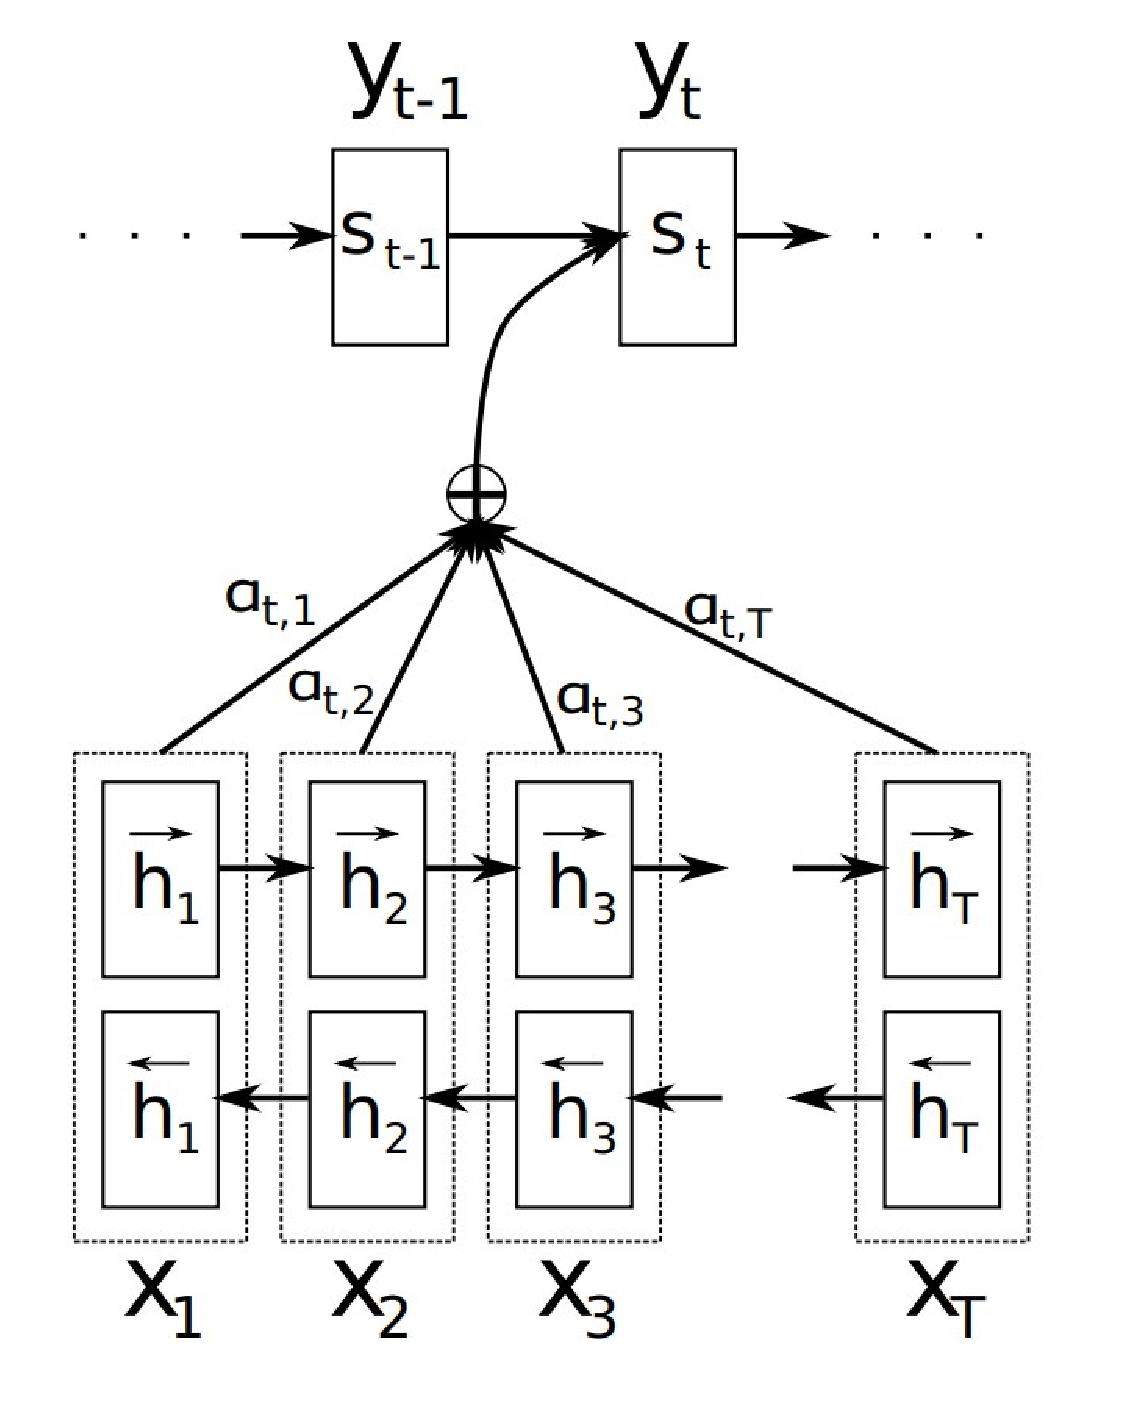
\includegraphics[width=9.5cm,height=9cm, clip=true]{./sources/attention.eps}
    \vspace{-10pt}
    \caption{\label{fig:attention} 注意力机制模型结构图}
    \vspace{-5pt}
\end{figure}

其中,$X$代表输入文本,$y$代表输出目标,定义如下条件概率:
\begin{equation}
    p(y_t|y_1, \dots, y_{t-1},x) = g(y_{t-1},s_i,c_i)
\end{equation}

其中,$s_i$代表第$i$时刻的RNN隐层单元,其计算公式如下:
\begin{equation}
    s_t= f(s_{t-1},y_{t-1},c_i)
\end{equation}
$c_i$依赖于来源于输入句子的隐藏序列$(h_1,\dots,h_{T_x})$,$c_i$由$h_i$加权求和得到:
\begin{equation}
a_{ij} = \frac{e_{ij}}{2\sum_{k=1}^{T_x}exp(e_{ik})}
\end{equation}

其中,$e_{ij}=a(s_{i-1},h_j)$,由前一时刻$s_{i-1}$和当前时刻隐层状态$h_j$构成。它是一个对其模型,代表输入数据位置$j$周围并且输出在位置$i$的匹配程度。

通过计算注意力机制,可以计算得到编码状态和解码状态之间的关联性权重,从而得到对当前输出位置比较重要的输入位置信息。本课题的研究同样使用了注意力机制用于支持判决预测任务。

\section{多任务学习}

多任务学习已经成功应用于机器学习的各个部分。多任务学习通过训练过程中包含在相关任务中的特定领域信息,提高模型的泛化性能。在自然语言处理深度学习领域,多任务学习通常包含隐层参数硬共享和隐层参数软共享两种。

\subsection{参数硬共享}
在硬参数共享是神经网络中最常用的方法。它通常用来在所有任务之间共享隐层参数,仅仅保持不同任务的输出层不同,其模型结果如图~\ref{fig:hard_share}:

\begin{figure}[htb]
    \centering
    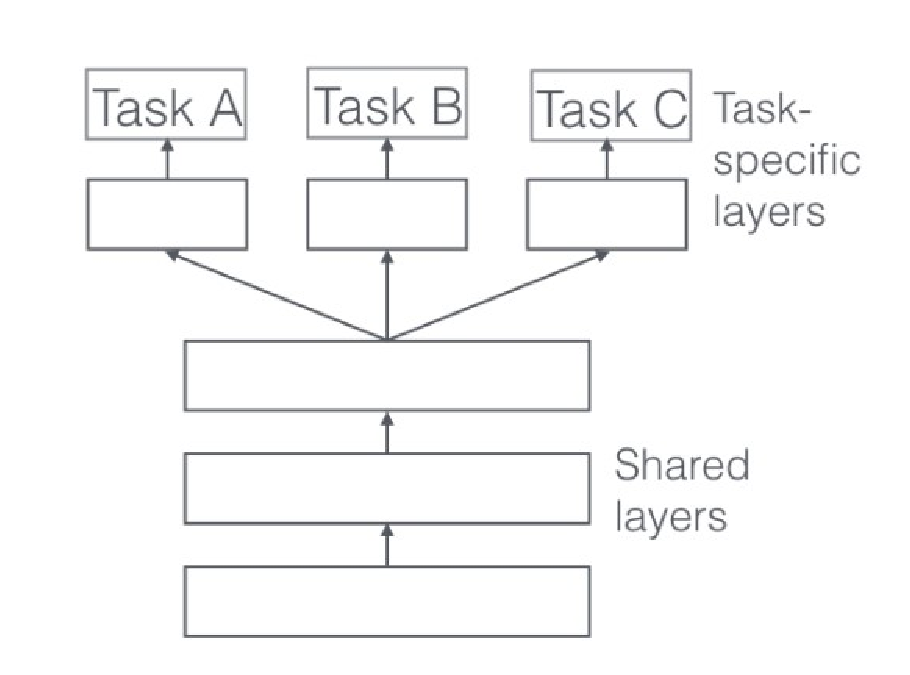
\includegraphics[width=11cm,height=7cm, clip=true]{./sources/hard_share.eps}
    \vspace{-10pt}
    \caption{\label{fig:hard_share} 参数硬共享模型结构图}
    \vspace{-5pt}
\end{figure}


参数硬攻向通常能很大程度上避免过拟合问题。我们同时学习的任务越多,我们的模型就需要学习到能代表所有任务的特征表达,因此我们的原始任务模型过拟合的几率就会越小。

\subsection{参数软共享}
在参数软共享模型中,每个模型都由自己的参数。不同模型参数之间的距离通过正则化来让共享层参数更加接近,其模型结构如图~\ref{fig:soft_share}:

\begin{figure*}[htb]
    \centering
    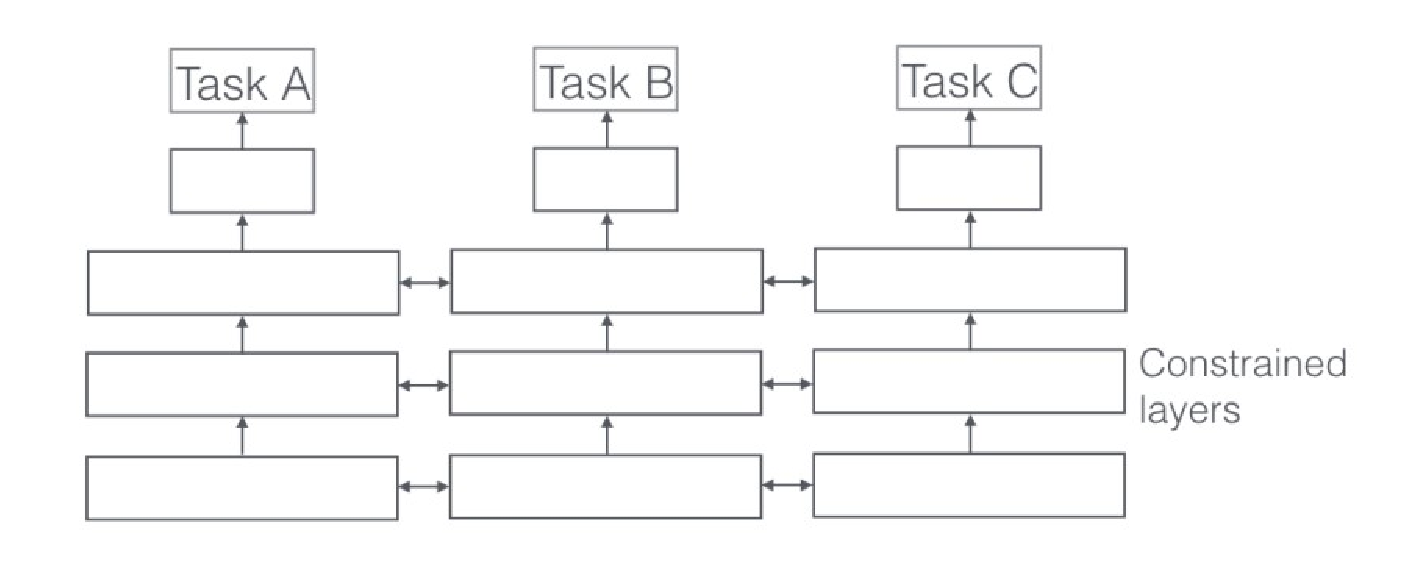
\includegraphics[width=14cm,height=6cm, clip=true]{./sources/soft_share.eps}
    \vspace{-10pt}
    \caption{\label{fig:soft_share} 参数软共享模型结构图}
    \vspace{-5pt}
\end{figure*}

在深度神经网络模型中,软参数共享中的约束层受到正则化的启发,已经用在了很多模型中。

多任务学习在我们训练过程中,有效地增加了训练样本的数量,所有的模型至少有一些噪声信息,当我们针对任务$A$训练模型时,我们的目标是针对任务$A$学习更好的表达,理想状态下忽略了噪声信息和泛化能力。不同的任务拥有不同的噪声模式,一个模型同时学习两个任务,可以学到更多泛化的表达。

\section{本章小结}
在本章节中,主要介绍了与本课题研究内容相关的一些基本概念,包括本课题研究内容问题的定义以及评价方法,还有本课题中用到的一些基本技术,包括文本表示方法,注意力机制与多任务学习。

% \chapterbib
